% !TEX root = ../main.tex

\section{Build System}
\label{sec:build_system}

Building the library and the EFM32 executables turned out to be one of the major parts of the work done in this project.
This section describes how building the project have changed over time.
This includes managing dependencies, compiling the {\core} library and \gls{rel}, and the Silicon Labs {\emlib}.
We have also utilized a continuous integration system that has helped us to keep the project up to date with the nightly builds of {\rust}, and to make sure that the builds have been consistent across the systems it has been built on.

\subsection{Manual Makefile}
\label{ssub:using_make}

When the project first started out it was based upon the \texttt{armboot}\footnote{\url{https://github.com/neykov/armboot/}} project available on GitHub.
\texttt{armboot} is a small template project for running {\rust} bare-metal on a STM32 ARM \glspl{mcu}.
These are, similarly with the EFM32 series, also based on the Cortex-M series of ARM processor cores.
We looked at \texttt{armboot}'s Makefile to figure out what flags to pass to {\rustc} in order to  cross-compile {\rust} programs for the ARM architecture.

\begin{table}[H]
  \centering
  \begin{tabular}{r|p{7cm}}
    \textbf{File} & \textbf{Description} \\
    \hline
    \file{thumbv7m-none-eabi.json} & Target specification for {\rustc}'s LLVM backend. \\
    \file{zero.rs} & Minimal {\rust} runtime requirements. \\
    \file{blinky.rs} & The executable program, it toggles the LEDs on the {\STK}. \\
    \file{efm32gg.ld} & EFM32 linker script. \\
    \file{startup\_efm32gg.s} & Defines the \code{ResetHandler} and the interrupt vector. \\
    \file{system\_efm32gg.c} & Used to manage the \gls{mcu} Clocks. \\
    \hline
  \end{tabular}
  \caption{Source files included in the first build for the ARM Cortex-M.}
  \label{tab:build:components}
\end{table}

\autoref{tab:build:components} lists the files included in the initial successful build\footnote{\url{https://github.com/havardh/geckoboot.rs/tree/8eb1df2417da0d7016d478de9cd011c98d77c592}} for the {\gecko}.
% The build process was contained within a manually developed Makefile.
The compilation process consisted of compiling the \file{blinky.rs} file to assembly by passing the target specification to the {\rustc} compiler.
This file was then, along with the \file{startup\_efm32gg.s} and \file{system\_efm32gg.c} files, compiled into object files with {\armgcc}, and linked into an executable with the \file{efm32gg.ld} linker script, using {\armld}.


% The build system was then was modified to include the \gls{rcl} library and initial bindings for {\emlib}.
% To do this the library was cross-compiled manually for the architecture producing a \file{libcore.rlib} library file.
% The initial bindings to {\emlib} were created inside the {\rust} source file and linked with \gls{rcl} before compiling to assembly.
% The {\C} implementation of the {\emlib} sources where compiled to object files like the \file{startup\_efm32gg.s} and \file{system\_efm32gg.c} files and all the object files are linked together.

After we had a working {\rust} program for the {\gecko} we included the \gls{rcl}, cross-compiled for ARM, and started to define peripheral bindings for {\emlib}.
The build system was later modified to generate the final executable with {\rustc} only, instead of generating an assembly file and compile it with {\armgcc}.
We could then use {\armgcc} to separately compile the {\emlib} source files into an archive, and link it with the final executable.
The three steps of this build routine is listed in \autoref{tab:build-steps}.

\begin{table}[H]
  \centering
  \begin{tabular}{p{7.5cm}|p{4cm}}
    \textbf{Build Step} & \textbf{Output} \\
    \hline
    \textbf{1)} Build {\emlib}, system, and startup with {\armgcc}. &
    Static {\C} archive. \\

    \textbf{2)} Cross-compile \gls{rcl} for ARM with {\rustc}. &
    Static {\rust} crate. \\

    \textbf{3)} Build the {\rust} bindings and the executable, and link it with the static libraries, generated from \textbf{1)} and \textbf{2)}, with the linker script. &
    Executable {\elf} file for the Cortex-M3. \\

    \hline
  \end{tabular}
  \caption{Early build routine.}
  \label{tab:build-steps}
\end{table}


% The final revision on the build system using Makefiles was to eliminate the assembly step for compiling the {\rust} sources.
% This was done by building an archive file for the object files generated by compiling the {\C} sources with the \cmd{arm-none-eabi-ar}, producing \file{libcompiler-rt.a}.
% The archive along with linker arguments was supplied to the {\rustc} compiler, when building the {\rust} source, in order to make the binary.
% Making this change resulting in the a build system with three steps as listed in \autoref{tab:build-steps}.

% \begin{table}[H]
%   \centering
%   \begin{tabular}{p{5.5cm} l l}
%     \textbf{Description}  & \textbf{Output} & \textbf{Output Type} \\
%     \hline
%     1. Building emlib+system+startup & \file{libcompiler-rt.a} & static archive \\
%     2. Building \gls{rcl} & \file{libcore.rlib} & static {\rust} crate \\
%     3. Building Rust source and linking executable & \format{\%.bin} & executable {\elf} file \\
%     \hline
%   \end{tabular}
%   \caption{Build steps}
%   \label{tab:build-steps}
% \end{table}

% At this stage of the evolution of the build system the {\emlib} bindings were build as part of the {\rust} application code.
% Later this was separated out to produce a \file{libemlib.rlib} which complements a \file{libemlib.a} containing the object files for the implementation of {\emlib}.
% By doing this also the system and startup code were separated to \file{libstartup.rlib} and \file{libstartup.a}.

\subsection{Transitioning to Cargo}
\label{ssub:transitioning_to_cargo}

It was always a goal to use {\cargo} for building, distributing, and managing the packages and dependencies that would become part of this project.
An obvious reason for this was to lower the bar for other potential users of the library, and to make our project as standalone as possible, so that it is easier to include and extend it as a part of other potential projects.
By letting {\cargo} handle as much as possible in its build routine, it would automate a lot of the work that every programmer using the library would otherwise have to do manually.

When the project first started out it was built by compiling {\rust}'s core library and the {\emlib} {\C} sources separately, and then linking them with the \gls{ffi} bindings by hand, as described in the previous section.
While this approach worked, it was far from optimal for a number of reasons:

\begin{itemize}
    \item {\rust} was in active development and many of its unstable \glspl{api} were going through rapid changes.
    Ensuring that versions of {\rustc} and the {\rust} source code stayed up to date across different systems was not easy.
    \item Compiling and ensuring that all dependencies were consistent across builds and systems for the bindings were a tedious task.
    A lot of the troubles concerning this came back to the point above.
    \item Linking dependencies with the library required each system to have set up several different \$PATHS to point to the right directories, what worked for one developer on one system might not have worked for different developer on another system.
    \item The {\cargo} package manager was developed for exactly these purposes among others.
\end{itemize}

As already described, {\cargo} is a tool that provides many operations to build {\rust} projects that have a certain project structure.
It is designed to integrate with other existing tools, like GNU Make, which has been important in  building this project.
When the transition to {\cargo} started, we focused on structuring the main library and its modules into the directory structure described in \autoref{ssub:project_structure}.
By invoking the \cmd{cargo build --verbose} command, it was possible to see the output from what {\cargo} attempted to build when it failed, and then structure the project accordingly.

A big priority was to to shrink the size of the makefiles that were in the project by making them a part of the standard build process for the {\rg} platform instead.
Doing this would help us get a long way of ensuring that the builds done by {\cargo} could be consistent across systems.
By defining a {\rust} build script and utilizing a {\rust} build-dependency called \prog{gcc}\footnote{\url{https://crates.io/crates/gcc}}, we were able to compile the {\C} sources from Silicon Labs' {\emlib} and link them with our bindings directly as part of the build process.
Note that the \prog{gcc} build-dependency is used as a shell to merely \emph{invoke} the underlying {\C}-compiler, in our case it is used to cross-compile with the {\armgcc} compiler.
By removing the dependency of manually compiling the {\C} sources, it was easier to start to automatically fetch the other dependencies, like the {\core} and \lib{collections} libraries.

Because this project is for a different processor architecture than the system that it is built on, we had to conditionally cross-compile all the standard {\rust} libraries that we wanted to utilize for the ARM Cortex-M3.
We could not utilize the pre-compiled libraries that are already included with {\rustc}, since these only works for the current system architecture.
This problem was solved by implementing a new {\cargo} build-dependency, called \texttt{rust-src}\footnote{\url{https://github.com/sondrele/rust-src}}, whose purpose is to download the entire {\rust} source code that is compliant with the instance of {\rustc} that is \emph{currently} compiling the library.
By making it a task for each build to fetch its own source code, we were guaranteed that the dependencies we used for the project would always compile, independent of the current instance of {\rustc} that was installed on the system.
The crates that we have fetched from {\rust}'s standard library that make up what we call \gls{rel} are already described in \autoref{sec:rel}, but they are also shown in \autoref{tab:compiled_libraries} for the sake of completeness.

\begin{table}[ht]
\begin{center}
\begin{tabular}{r|p{8cm}}
\textbf{Rust library} & \textbf{Purpose} \\
\hline
\lib{core}        & {\rust}'s core library that declares basic types. \\
\lib{libc}        & Types to use with {\rust}'s \gls{ffi}. \\
\lib{alloc}       & Allows for heap-allocated variables. \\
\lib{collections} & Provides common collections like dynamically allocated Strings and Vectors. \\
\lib{unicode}     & Required by collections for e.g. Strings. \\
\lib{rand}        & Generate random values. \\
\hline
\end{tabular}
\caption{{\rust} libraries conditionally compiled for the Cortex-M3 architecture.}
\label{tab:compiled_libraries}
\end{center}
\end{table}

By design, {\cargo} only supported passing two flags further on to {\rustc}, those were \flag{-L} and \flag{-l}.
The purpose of these flags is to tell {\rustc} to link with an external library by looking in a directory (specified with the \flag{-L} flag), for a library with the specified name (specified with the \flag{-l} flag).
The last step in the build process involved linking the bindings and the other libraries with an actual executable for the Cortex-M3.
This was not possible to do with {\cargo} since it required us to pass a couple of extra linker-flags further on to {\rustc}.
The flags were needed by {\rustc} in order to tell it to link with an external library for a different architecture and to include a separate linker-script that took care of booting up the executable on this architecture.

Another issue that was introduced by automatic compilation with {\cargo}, was how it structured the packages it compiled.
When {\cargo} builds a project and its dependencies, it structures all the generated metadata and the compiled libraries within a \dir{target} directory, and an extra filename gets appended to all of these libraries.
This extra filename is part of a hash that is generated based on the code in the library.
It ensures that each and every build is consistent and it resolves any problems that might arise if several dependencies within a project depend on different versions of the same library.
This works when {\cargo} handles the entire build process, but it our case, where we had to manually compile the final executable, it turned out to be a problem because the name of the library would change every time some of its content changed.
We worked around this problem by modifying the build script to store the hash generated by {\cargo} for {\emlib} to a separate file, every time the library was built, and then included it in the makefile for the project.

\subsection{Conditional linking with Cargo}

The build process described in the previous section made it simpler to use third party libraries, but it did not solve all of our issues.
The main problem that persisted was to have a good way of making the bindings themselves portable.
With the setup that we had, it was easy to create new executables \emph{within} the project, but it was hard to create new executables that \emph{depended} on the bindings.
Basically, because we had to work around {\cargo} in the final part of the build process, it also meant that \emph{every} project that wanted to depend on {\emlib} also had implement the same workarounds.
Thus, we needed to solve the problem of knowing where {\cargo} would store the project metadata, and we needed a way to get {\cargo} to compile the final executables with the extra linker-arguments needed by {\rustc} in order to compile the binary for the Cortex-M3.

{\cargo} does not have much documentation over how its internal works, or how to interfere with the build process, but the documentation does mention that {\cargo} can be extended with additional \emph{plugins}.
If {\cargo} is to be invoked with a command that it does not have by default, it will query the system for this command.
This means that if {\cargo} is invoked with e.g. the command \cmd{cargo foo <args>...}, it will query the system for an executable with the name \file{cargo-foo} and it will invoke this command with the trailing arguments if it exists.
By looking at {\cargo}'s source code, we could see that every triggered build included a structure called \code{CompileOptions}.
The arguments passed to {\cargo}'s different build commands are then used to compose this structure and trigger an internal compilation process.
This process handles the compilation of all dependencies and generates all the different binaries for the current package to be compiled.

\begin{table}[ht]
\begin{center}
\begin{tabular}{r|p{8cm}}
\textbf{Flags} & \textbf{Purpose} \\
\hline
\texttt{[$<$args$>$]} &
The trailing argument to the command was the linker-arguments that were to be passed further on to the invocation of {\rustc}.
If any \emph{args} are present, {\cargo} will append \flag{-C link-args="$<$args$>$"} when any executables from the package is being built. \\

\flag{--examples NAME} &
The library had many executables located in the projects \dir{examples} directory.
This flag made it easier to compile one of these examples by specifying its name. \\

\flag{--build-examples} &
This flag filtered out every executable marked as an example and compiled all of them. \\

\flag{--print-link-args} &
This flag was included for debugging purposes. \\

\hline
\end{tabular}
\caption{}
\label{tab:cargo_linkargs}
\end{center}
\end{table}


In order to solve the problems we had with building the project, we created a new subcommand called \cmd{cargo-linkargs}\footnote{\url{https://github.com/RustyGecko/cargo-linkargs/}} that depends on {\cargo} itself.
This subcommand was created specifically with {\rg} in mind, and supports all the flags that the \cmd{cargo-build} command supports, including the flags shown in \autoref{tab:cargo_linkargs}.
We got rid of the two problems we had with building the {\rg} platform once \cmd{cargo-linkargs} was working.
The problem with resolving the location of generated metadata was solved implicitly just by utilizing {\cargo}, and the extra linker-arguments could easily be passed on to the invocation of \cmd{cargo-linkargs} via the project's makefile.

\subsection{Continuous Integration}
\label{ssub:continuous_integration}

When we first started this project, {\rust} had reached a 1.0-alpha version.
This meant that the programming language had reached a relatively stable state, but there was still big parts of the language and its standard libraries that were marked as unstable and up for review before the planned 1.0 release.
The standard libraries, and third-party {\rust} libraries that have evolved in the {\rust} community, have made small guarantees about their stability, and the \glspl{api} have been subject to change without much notice.

Continuous Integration refers to the practice of testing the whole system \emph{continuously}, for every smaller change introduced to the code base, usually with an automated test framework.
Continuous Integration is advantageous to normal regression testing because it can reduce the amount of code rework that is needed in later phases of development, as well as speed up overall development time  \cite{Orso2014}.
Many {\rust} projects have utilized a continuous integration system called Travis CI\footnote{\url{https://travis-ci.com/}} for ensuring that the code in the project has been compatible with the nightly builds of {\rust}.
By registering our projects with Travis CI, and a community-developed service called {\rust} CI\footnote{\url{http://rust-ci.org/}}, we had automatic, daily builds of our projects on a third-party server.
Builds were triggered every time we released a change to the code on GitHub, and every time a new nightly release of {\rust} was published.
And if a build failed we would get notified of the error.
By making continuous integration part of the normal build routine and review process for new project code, we had an extra step of verification that the project would build on other systems then the one it was developed on.

It is important to note that continuous integration only helped us to verify that the project could be \emph{built}, it could not help us to prove that the compiled code would actually \emph{work} for its target architecture.
To verify that the code would work for the Cortex-M3, we had to run in on one of the \glspl{mcu} that we had available for this project.
An experimental process of testing and mocking the {\rg} bindings is described in greater detail in \autoref{ssub:testing}.

\subsection{Contributing to Cargo}
\label{ssub:contributing_to_cargo}

As already mentioned, the ability to pass arbitrary flags further on to the invocation of {\rustc} was by design not supported by {\cargo}.
However, many people in the {\rust} community have wanted the ability to do so.
The reasoning for not allowing arbitrary flags to be passed down is described in this section.

A compilation can go awry very quickly if it is up to the package \emph{author} what flags should be passed to {\rustc}.
Instead, it should be up to the \emph{user} of the package.
This would have given the author the ability to set the restriction for a library, and limit the possibilities of what a user could have done with it.
Different systems do not necessarily support all flags and possibilities.
Thus, if a package dependency says that it is to be built in a particular way, it might not work on the system it is being built for.

On the {\cargo} project's issue tracker, several related issues concerning passing arbitrary flags further on to {\rustc}, was open.
All these were formalized in one issue\footnote{\url{https://github.com/rust-lang/cargo/issues/595}} for implementing a new subcommand (called \cmd{cargo-rustc}) for the package manager.
This subcommand would have allowed for passing these flags on to {\rustc}, but with the restriction of only compiling a \emph{single} binary at a time.
This means that only \emph{either} the library, a binary, an example or a test (or a package dependency), may be compiled with the extra flags, and \emph{not} the entire package.

These rules are restrictive enough to get libraries to not depend on a set of extra flags, but loose enough so that specialized projects, like our bindings, can depend on it for completing the build.
Indeed, the functionality proposed with this subcommand would be enough to cover all the cases that we solved with our implementation of \cmd{cargo-linkargs}.

After gaining insight into {\cargo}'s internals during the development of \cmd{cargo-linkargs}, it was interesting to see if we could get this same functionality into {\cargo} itself, by implementing \cmd{cargo-rustc}.
Even though \cmd{cargo-linkargs} worked great for its purpose, it was not very ergonomic for {\rg} to depend on a third-party plugin to work.
Especially if {\cargo} could natively support this functionality.
Not only would it benefit our project, it would also give many other {\rust} projects the ability to use {\cargo} for the entire compilation process.
Since both {\rust} and {\cargo} are open source projects, it was quick to get in contact with the project maintainers about the issue, and eventually submit a patch with the new subcommand.
After it had been reviewed by one of the project maintainers, the patch was accepted and merged into {\cargo}'s code base.
The subcommand developed as part of our build system is now a part of {\rust}'s nightly builds.

\subsection{Final Library Build Artifacts}

The resulting files of compiling the libraries are presented in \autoref{fig:lib:structure}.

\begin{figure}[H]
  \begin{center}
    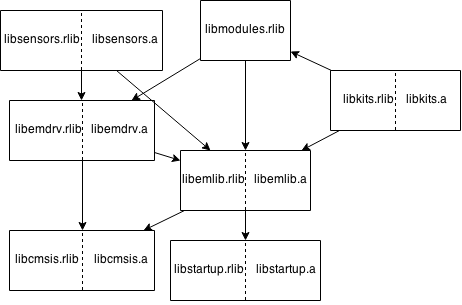
\includegraphics[scale=0.5]{figures/lib-structure.png}
  \end{center}
  \caption{The organization files of libraries}
  \label{fig:lib:structure}
\end{figure}

The figure shows that all of the libraries except for \lib{modules} consists of both a {\C} static archive (\format{*.a}) and a {\rust} library (\format{*.rlib}).
The \lib{modules} library is a high level library that is built on top of the bindings for {\emlib} and {\emdrv}, and its implementation is described in \autoref{sec:rust-embedded-modules}.
The rest of the libraries provides {\rust} bindings in the \format{*.rlib} part and the {\C} implementations in the \format{*.a} portion.
We also see the dependencies, denoted by the arrows, between the libraries, generally flowing from the top level abstraction down to the lower level abstractions.
